\subsubsection{Front}
Un peu plus intéressant que l'opérateur S, l'opérateur front, abrégé {\em F} dans Taggre, va limiter le nombre de tâche disponible au même moment dans l'ordonnanceur.
%
Pour cela, il va travailler à diminuer la largeur du graphe.
%
Certaines propriétés du graphe peuvent être corrélées aux résultats de l'ordonnanceur.
%
Par exemple, la hauteur d'un graphe correspondra au temps minimum qu'il faudra pour traiter tout le graphe si nous avons un nombre infini d'unité de calcul.
%
La largeur du graphe donnera un indice sur le parallélisme exploitable.
%
Plus un graphe est large, plus il offrira de parallélisme.
%
En effet, avec un nombre illimité de coeur de calcul, on peut exploiter au mieux le même nombre de coeur que la largeur du graphe.
%
Le cas idéal serait donc un graphe d'une tâche de hauteur avec un nombre conséquent de tâche à la même hauteur.
%
Ce cas ressemble fortement au parallélisme de boucle.
%
Le nombre de tâches du graphe est aussi une propriété à prendre en compte, l'ordonnanceur doit pouvoir stocker toutes les tâches dans des structures de données.



Un graphe fournissant énormément de parallélisme par rapport au nombre de coeur disponible n'aura pas forcément un meilleur équilibrage de charge par rapport à un graphe offrant moins de parallélisme.
%
D'autre part, trop de parallélisme peut conduire à la congestion des structures de données servant à maintenir à jour les tâches prêtes à être ordonnancer.
%
En réduisant la largeur du graphe, on peut ainsi réduire le parallélisme.
%
Mais il faut faire attention à ne pas trop le réduire.
%
C'est pourquoi l'opérateur F prend en paramètre la largeur du graphe souhaitée.
%
L'algorithme de l'opérateur F consiste à parcourir le graphe par hauteur et de limiter le nombre de tâches par hauteur à un paramètre donné par le programmeur (Algo.~\ref{algo:algo_F}).
%
Seules les tâches qui ont la même hauteur sont agrégées ensemble, il n'y a donc aucun risque de création de cycle (Fig.~\ref{fig:algo_F2}).


%   (-_-)   %
\begin{figure}[t!]
  \centering
  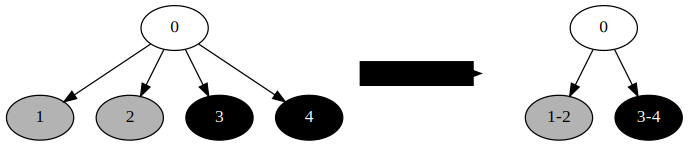
\includegraphics[width=0.7\textwidth]{algo_F2}
  \caption{Exemple d'agrégation avec l'opérateur F et le paramètre 2.}
  \label{fig:algo_F2}
\end{figure}

\begin{algorithm}
  \KwData{$M$, DAG}
  {\sc Suivant} = liste vide \\
  mettre les tâches racines de DAG dans {\sc Suivant} \\
  \While{{\sc Suivant} n'est pas vide} {
    {\sc Prêt} = {\sc Suivant} \\
    {\sc Suivant} = liste vide \\
    {\sc Moyenne} = 0 \\
    \For{chaque tâche {\sc T} de {\sc Prêt}} {
      {\sc Moyenne } += taille de {\sc T}
    }
    {\sc Moyenne} /= taille de {\sc Prêt} \\

    \While{{\sc Prêt} n'est pas vide} {
      mettre les successeurs des {\sc Moyenne} premières tâches dans {\sc Suivant} \\
      agréger les {\sc Moyenne} premières tâches de {\sc Prêt} \\
      retirer les {\sc Moyenne} premières tâches de {\sc Prêt}
    }
  }
  \caption{Algorithme de l'opérateur front.}
  \label{algo:algo_F}
\end{algorithm}
